\documentclass[../Calculus_\Roman{3}]{subfiles}

\begin{document}
	\section{Three-Dimensional Coordinate Systems}
		Any point in a plane can be represented as an ordered pair of real numbers. Because this uses two numbers, a plane is called two-dimensional. To locate a point in space, a triplet of real-numbers is required.
		\subsection*{3D Space}
			\addcontentsline{toc}{subsection}{3D Space}
			Before points can be represented in 3D space, a fixed point $O$ (the origin) and three perpendicular lines that pass through it, called the \textbf{coordinate axes}. These axes are labeled the $x$-, $y$-, and $z$-axes. In general, the former two are horizontal while the third is vertical. The direction of the $z$-axis is determined by the \textbf{right-hand rule}. Curling the fingers of the right hand from the positive $x$-axis to the positive $y$-axis, the thumb will point in the direction of the positive $z$-axis. \\
			The three coordinate axes determine the three \textbf{coordinate planes}.
			\[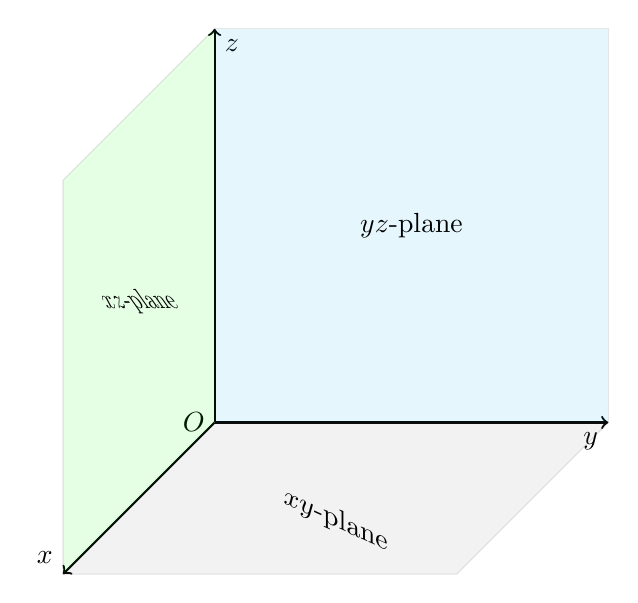
\begin{tikzpicture}[xscale = 5, yscale = 5]
				\coordinate (O) at (0, 0, 0) node[anchor = east]{$O$};
				\draw[thick, ->] (0, 0, 0) -- (1, 0, 0) node[anchor = north east]{$y$};
				\draw[thick, ->] (0, 0, 0) -- (0, 1, 0) node[anchor = north west]{$z$};
				\draw[thick, ->] (0, 0, 0) -- (0, 0, 1) node[anchor = south east]{$x$};
				\draw[fill = cyan, opacity = 0.1] (0, 0, 0) -- (1, 0, 0) -- (1, 1, 0) -- (0, 1, 0);
					\node at (0.5, 0.5, 0) {$yz$-plane};
				\draw[fill = green, opacity = 0.1] (0, 0, 0) -- (0, 1, 0) -- (0, 1, 1) -- (0, 0, 1);
					\node[xslant = -0.7, xscale = 0.7] at (0, 0.5, 0.5) {$xz$-plane};
				\draw[fill = gray, opacity = 0.1] (0, 0, 0) -- (0, 0, 1) -- (1, 0, 1) -- (1, 0, 0);
					\node[below, yslant = -0.45] at (0.5, 0, 0.5) {$xy$-plane};
			\end{tikzpicture}\]
			Three planes divided space into eight \textbf{octants}. Illustrated above are the positive $xz$-, $yz$-, and $xy$-planes, constituting the \textbf{first octant}. \\
			A point's \textbf{coordinates} are an ordered triple of real numbers. A point's \textbf{projection} onto a plane is the point with two of the same coordinates, the third becoming 0.
			\[\begin{array}{|c|c|c|c|}\hline
				\text{Plane} & xy & yz & xz \\\hline
				(a, b, c) & (a, b, 0) & (0, b, c) & (a, 0, c) \\\hline
			\end{array}\]
			The set of all ordered triples is the cartesian product of three sets of all real numbers, denoted appropriately by $\mathbb{R}^3$ and defined as
			\[\mathbb{R}^3 = \mathbb{R} \times \mathbb{R} \times \mathbb{R} = \{(x, y, z) \mid x, y, z \in \mathbb{R}\}\]
			A one-to-one correspondence between points in space and ordered triples in $\mathbb{R}^3$ is a \textbf{three-dimensional coordinate system}. It should be noted that the first octant can be described as the set of points for which all coordinates are positive.
			\subsection*{Distances and Spheres}
				\addcontentsline{toc}{subsection}{Distances and Spheres}
			\callout{17}{
				\paragraph{Distance Formula in Three Dimensions} The distance $|P_1P_2|$ between points $P_1(x_1, y_1, z_1)$ and $P_2(x_2, y_2, z_2)$ is
				\[|P_1P_2| = \sqrt{(x_2 - x_1)^2 + (y_2 - y_1)^2 + (z_2 - z_1)^2}\]
			}
			\callout{17}{
				\paragraph{Equation of a Sphere} 
					The equation of a sphere with center $(h, k, l)$ and radius $r$ is
					\[(x - h)^2 + (y - k)^2 + (z - l)^2 = r^2\]
			}
		\section{Vectors}
\end{document}